\documentclass{article}
\usepackage{ctex}
\usepackage{graphicx}
\usepackage{amsmath}
\usepackage{indentfirst}
\usepackage{titlesec}
\usepackage{setspace}
\usepackage{subfigure}
\usepackage{caption}
\usepackage{float}
\usepackage{booktabs}
\usepackage{geometry}
\usepackage{multirow}
\geometry{left=1.2cm,right=1.2cm,top=2cm,bottom=2cm}
\title{\songti \zihao{2}\bfseries 闪烁体荧光时间特性的观测与分析预习报告}
\titleformat*{\section}{\songti\zihao{4}\bfseries}
\titleformat*{\subsection}{\songti\zihao{5}\bfseries}
\renewcommand\thesection{\arabic{section}}
\author{王启骅 PB20020580}
\begin{document}
	\maketitle
	\section{实验目的}
	1.学会正确使用数字示波器来分析闪烁计数器的输出脉冲波形。
	
	
	2.学会根据记录的波形了解闪烁体的时间特性。
	
	\section{实验装置}
	1.记录单次脉冲的数字存储示波器。
	
	
	2.可切换闪烁体的闪烁计数器系统,包括高压电源。
	
	
	3.契仑可夫辐射体(有机玻璃),NaI(Tl),CsI(Tl),塑料闪烁体,氟化铈晶体(CeF3)。
	
	\section{实验原理}
	闪烁计数器是一种应用非常广泛的重要粒子探测器,它由闪烁体、荧光光子检测器两个
	基本元件组成。
	
	
	1. 闪烁体: 主要是塑料闪烁体以及各种无机闪烁晶体。例如: NaI(Tl)晶体、CsI(Tl)
	晶体、锗酸铋晶体(BGO)等。它们的作用是将通过闪烁体的粒子($ \alpha、\beta、\gamma  $以及 $ \mu $ 子、$\pi$ 介
	子等)沉积的能量转换成闪烁荧光光子。
	
	
	2. 荧光光子检测器: 包括各种光敏检测器,最常用的是光电倍增管。光电倍增管的
	作用是将闪烁体输出的荧光光子转换成光电子,并对原初光电子进行倍增,最后在光电倍增
	管的阳极输出回路上形成一个与输入的荧光脉冲相对应的电流脉冲。过程见图1。
	
	\begin{figure}[!h]
		
		\centering
		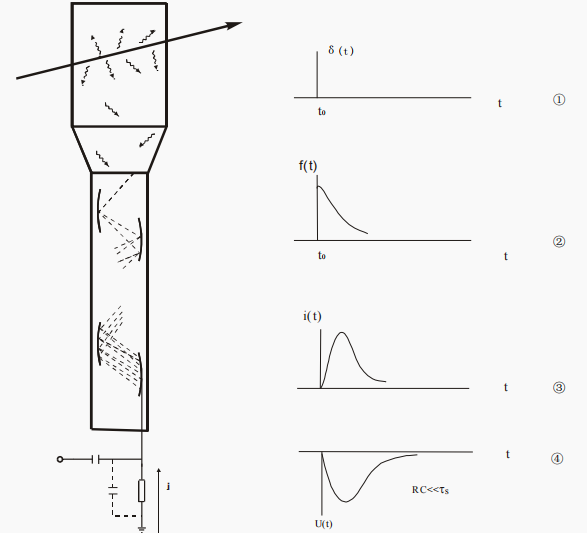
\includegraphics[scale=0.7]{原理}
		\captionsetup{font={small},labelfont=bf}
		\caption{\heiti\zihao{-5}闪烁体时间特性实验原理图}
		
	\end{figure}
	
	
	图 1 中:
	
	
	图(1):粒子通过闪烁体与闪烁体原子、分子发生相互作用,沉积能量。这种过程持续时
	间为皮秒($ 10^{-12}s $)量级,能量沉积响应近似为$ \delta_(t_0)。 $
	
	
	图(2):沉积的能量在闪烁体中激发形成闪烁荧光发光中心,过程近似为$ \delta_(t_0) $,之后发
	光强度随时间的变化 f(t)依时间常数$ \tau_S $按指数衰减,$ \tau_S $ 与闪烁体的荧光发射机制有关。例
	如 NaI(Tl)晶体$ \tau_S \sim 230ns $,BGO:$ \tau_S \sim 300ns $, 塑料闪烁体:$ \tau_S\sim1-2ns $。有的闪烁体荧
	光的时间过程由多种时间常数决定。若光在闪烁体中的传输和收集时间忽略不计,(2)中
	$t_0'\sim t_0$。
	
	
	图(3):光电倍增管阳极单位时间收集电子数随时间变化。由于光阴极光电转换过程和各
	打拿极的倍增过程的时间晃动和时间延迟,单位时间电子数脉冲形状仅近似为荧光脉冲形
	状,前沿由于度越时间的分散而上升变慢,后沿衰减时间常数$ \tau $近似为$\tau_S$,它携带着闪烁
	体的荧光时间特性的信息。所以它是荧光时间分布在时间轴上移动了 $ t_d $ 后与光电倍增管单
	光子度越时间分布函数的卷积。
	
	\begin{equation}
		f(t+t_d)\odot T_s(t)=n_e(t)
	\end{equation}
	\begin{equation}
		i(t)=\dfrac{dn_e}{dt}
	\end{equation}
	
	
	图(4):光电倍增管的输出电压脉冲波形U(t),是电流脉冲$ i=\dfrac{dn_e(t)}{dt} $在光电倍增管的输出RC回路上形成的。通过解电路方程,可求出输出电压U(t)。对$ i(t)=i_0\exp(-\frac{t}{\tau_s})=\frac{Q_0}{\tau_s}\exp(-\frac{t}{\tau_s}) $
	
	\begin{equation}
		U(t)=\frac{Q_0 R}{RC-\tau_s}\big(\exp(-\frac{t}{RC})-\exp(-\frac{t}{\tau_s})\big)
	\end{equation}
	其中 RC 为输出回路时间常数,$ Q_0 $为阳极收集的总电荷,$\tau_s$ 为荧光脉冲的衰减时间常数。
	通过已知衰减时间常数的晶体得到的输出波形,拟合求得输出回路的 RC(标定系统的 RC)。
	标定系统的 RC 之后,可以根据测得的波形,用公式(1)来拟合,就能定出闪烁体的荧光
	时间特性。在 $ RC<<τ_S $情况下,由式(1)可以得到
	\begin{equation}
		U(t)=-\frac{Q_0 R}{\tau_S}\big(\exp(-\frac{t}{RC})-\exp(-\frac{t}{\tau_s})\big)
	\end{equation}
	
	
	另一种观测闪烁体荧光衰减的方法是图 A 的闪烁体以下的部分看成一个系统,先用契
	伦柯夫辐射作为$\delta$光源直接照射光阴极,记录输出脉冲波形,该脉冲波形就是系统对$\delta$光源
	的响应函数 *(t)。用闪烁体取代契伦柯夫辐射体(有机玻璃),设闪烁体的荧光时间分布
	f(t),则其输出波形为
	
	\begin{equation}
		W(t)=f(t)\odot\delta(t)
	\end{equation}
退卷积可得到f(t)。
	\section{实验内容}
	1.观测闪烁体荧光时间特性对输出波形的影响,辨认快慢闪烁体。
	
	
	2.观测光电倍增管输出回路的时间常数对输出脉冲波形的影响。
	
	
	3.用$\delta$光源测定光电倍增管的响应函数* (t)。
	
	
	4.分析记录不同闪烁体的荧光衰减时间常数$ \tau_S $。
	\section{实验步骤}
	1.选择1$ \# $样品有机玻璃,设定光电倍增管输出回路R=50$ \Omega $。
	
	
	2.加光电倍增管高压至规定值。
	
	
	3.在数字示波器上记录宇宙线通过样品产生的脉冲波形,记录存储10个事例的波形。
	
	
	4. 分别置入其它样品,同样记录存储10个波形。
	
	
	5. 置入NaI(Tl)晶体,改变输出回路的负载电阻,在每种RX参数下记录5个波形。
	

	\section{数据处理}
	1.根据输出的波形数据,以NaI(Tl)晶体的波形为参考,设$ \tau_S $=250ns,由式(3)拟合出输
	出回路的RC。
	
	
	2. 用已知的RC将其它样品的波形与式(3)拟合,求各个样品的$ \tau_S $。


	3. 用1$ \# $样品的输出波形作为响应函数* (t),通过退卷积求出各样品的f(t)。
	
	
	4.对实验步骤⑤的数据(R=1M$ \Omega $),通过对输出波形的后沿的拟合,求出输出回路的分布
	电容C。
\end{document}